\documentclass[preprint]{sigplanconf}

\usepackage{amsfonts}
\usepackage{amsmath}
\usepackage{natbib}
\usepackage{graphicx}
\usepackage{tikz}
\usepackage{mathtools}
\usetikzlibrary{chains,fit,shapes,calc}
\usepackage{verbatim}
\usepackage{semantic}
\usepackage{tabu}
\usepackage{amsthm}
\usepackage{mathptmx}
\usepackage{todonotes}
\newcommand{\concat}{\ensuremath{+\!\!\!\!+\,}}  

\newtheorem{prop}{Proposition}
\newtheorem{lemma}{Lemma}
\newtheorem{defin}{Definition}

\begin{document}

\conferenceinfo{IFL '15}{September 14-16, 2015, Gothenburg, Sweden} 
\copyrightyear{2015} 
\copyrightdata{[to be supplied]} 

\titlebanner{Preprint}        % These are ignored unless
\preprintfooter{Cactus Environment Machine}   % 'preprint' option specified.

\title{Cactus Environment Machine}
\subtitle{Shared Environment Call by Need}

\authorinfo{George Stelle}
           {University of New Mexico}
           {stelleg@cs.unm.edu}
\authorinfo{Darko Stefanovic}
           {University of New Mexico}
           {darko@cs.unm.edu}
\authorinfo{Stephen L. Olivier}
           {Sandia National Laboratories}
           {slolivi@sandia.gov}
\authorinfo{Stephanie Forrest}
           {University of New Mexico}
           {forrest@cs.unm.edu}

\maketitle

\begin{abstract}
Existing machines for lazy evaluation use a \emph{flat} representation of
environments, storing the terms associated with free variables in an array.
Combined with a heap, this structure supports the shared intermediate
results required by lazy evaluation.  This paper proposes and describes an
alternative approach that uses a \emph{shared} environment to implement lazy
evaluation.  We show how a shared environment can act as both an environment and
a mechanism for sharing results. To formalize this approach, we describe a novel
calculus that makes the shared environment explicit, as well as a machine to
implement the calculus: the \emph{Cactus Environment Machine} ($\mathcal{CE}$
machine). A simple compiler implements the machine and is used to run
experiments for assessing performance.  The results show reasonable performance
and suggest that with the addition of some common optimizations, the
$\mathcal{CE}$ machine could be competitive with existing high performance lazy
evaluation implementations.
%In addition, we implement a simple compiler that targets native
%code and show that it has reasonable performance despite some significant
%but addressable shortcomings.
\end{abstract}

\section{Introduction}

Call-by-need evaluation is a formalization of the idea that work
should be delayed until needed, and performed only once.  Existing
implementations of call-by-need take care in \emph{packaging} a delayed
computation, or \emph{thunk}, by building a closure with an array that contains
the bindings of all free variables \cite{jonesstg,boquist1997grin}. The overhead
induced by this operation is well known, and one reason existing implementations
avoid thunks wherever possible \cite{johnsson1984efficient}. The key insight of
our Cactus Environment ($\mathcal{CE}$) Machine is that this overhead can be
minimized by only recording a location in a shared environment.

As an example, consider the application $f \; e$. In existing call-by-need
implementations, e.g., the STG machine\cite{jonesstg}, a closure with a flat
environment will be constructed for $e$.  Doing so incurs a time and memory cost
proportional to the number of free variables of $e$. \footnote{In some
implementations, these are lambda lifted to be formal parameters, but the
principle is the same.} We minimize this packaging cost by recording a
location in a shared environment, which requires only two
machine words (and two instructions) for the thunk: one for the code pointer,
and one for the environment pointer. One way to think about the approach is that
it is \emph{lazier} about lazy evaluation: in the case that $e$ is unneeded, the
work to package it in a thunk is entirely wasted. In the spirit of lazy
evaluation, we attempt to minimize this potentially unnecessary work.  

The main contributions of the paper are:
\begin{itemize}
\item A big-step calculus and small-step abstract machine that formalize the
notion of a shared environment for call-by-need evaluation using an explicitly
shared environment (Section~\ref{sec:calc}).
\item A simple implementation of the abstract machine that compiles to x86
assembly with a preliminary evaluation that shows performance comparable to
existing implementations (Sections~\ref{sec:impl} and~\ref{sec:eval}).
\end{itemize}

Section~\ref{sec:back} reviews relevant background material, and
Section~\ref{sec:env} discusses the current landscape of environment
representations, highlighting the opportunity for combining shared environments
with lazy evaluation.  We then provide some intuition for why this combination
is desirable, and formalize the connection between call-by-need evaluation and
shared environments in a calculus (Section~\ref{sec:calc}).
Section~\ref{sec:mach} uses the calculus to derive a novel abstract machine, the
$\mathcal{CE}$ machine, explains how $\mathcal{CE}$ uses the shared environment
in a natural way to implement lazy evaluation, and gives its formal semantics.
We then describe a straightforward implementation of $\mathcal{CE}$ in
Section~\ref{sec:impl}, extended with machine literals and primitive operations,
compiling directly to native code. We evaluate the implementation in
Section~\ref{sec:eval}, showing that it is capable of performing comparably to
existing implementations, despite lacking several common optimizations, and
discuss the results. We discuss related work, the limitations of our approach,
and some ideas for future work in Section~\ref{sec:disc}, and conclude the
paper in Section~\ref{sec:conc}.



\section{Background and Motivation} \label{sec:back}

This section provides relevant background for the $\mathcal{CE}$ machine,
outlining lambda calculus, evaluation strategies, and Curien's calculus of
closures.

\subsection{Preliminaries}

We begin with the simple lambda calculus ~\cite{barendregt1984lambda}:  $$ t::= x
\; | \;  \lambda x.t \; | \;  t \; t $$ where $x$ is a variable, $\lambda x.t$
is an abstraction, and $t \; t$ is an application. We also use lambda calculus
with deBruijn indices, which replace variables with a natural number indexing
into the binding lambdas.  This calculus is given by the syntax: $$ t::= i \; |
\; \lambda t \; | \; t \; t $$ where $i \in \mathbb{N}$. In both cases, we use
the standard Barendregt syntax conventions, namely that applications are left
associative and the bodies of abstractions extend as far as possible to the
right ~\cite{barendregt1984lambda}.  A \emph{value} in lambda calculus refers to
an abstraction. We are concerned only with evaluation to weak head normal form
(WHNF), which terminates on an abstraction without entering its body.

In mechanical evaluation of expressions, it would be too inefficient to perform
explicit substitution. To solve this, the standard approach uses closures
~\cite{landin1964mechanical,curien1991abstract,jonesstg,biernacka2007concrete}.
Closures combine a term with an environment, which binds the free variables in
the term to closures. 

For a formal basis for closures, we use Curien's calculus of
closures~\cite{curien1991abstract}, given in Figure~\ref{fig:calcclos}.  It is a
formalization of closures with an environment represented as a list of closures,
indexed by deBruijn indices. We will occasionally modify this calculus by
replacing the deBruijn indices with variables for readability, in which case
variables are looked up in the environment instead of indexed, e.g., $t[x = c, y
= c'])$ ~\cite{barendregt1984lambda}. We also add superscript and subscript
markers to denote unique syntax elements, e.g., $t', t_1 \in \textnormal{Term}$. 

\subsection{Evaluation Strategies} \label{sec:eval}

There are three standard evaluation strategies for lambda calculus:
call-by-value, call-by-need, and call-by-name.  Call-by-value evaluates every argument
to a value, whereas call-by-need and call-by-name only evaluate an argument if
it is needed.  If an argument is needed more than once, call-by-name re-computes
the value, where call-by-need memoizes the value, so it is computed at most once.
Thus, call-by-need attempts to embody the best of both worlds---never repeat
work (call-by-value), and never perform unnecessary work (call-by-name). These
are intuitively \emph{good} properties to have, and we illustrate the
correctness of such an intuition with the following example, modified from
~\cite{danvy2013synthetic}:

$$ \overbrace{c_m (c_m (\cdots(c_m}^{m} \; id \; \overbrace{id)\cdots) id)}^{m} \; true \; id
\; bottom $$ where $c_n = \lambda s.\lambda z.\overbrace{s \; (s \cdots (s}^{n}
\; z) \cdots) $, $true = \lambda t.\lambda f.t$, $id=\lambda x.x$, and $bottom =
(\lambda x.x \; x) \lambda x.x \; x$. Call-by-value never terminates,
call-by-name takes exponential time, and call-by-need takes only polynomial time
~\cite{danvy2013synthetic}. Of course, this is a contrived example, but it
illustrates desirable properties of call-by-need.

In practice, however there are significant issues with call-by-need evaluation.
We focus on the following: \emph{Delaying a computation is slower than
performing it immediately.} This issue is well known
\cite{johnsson1984efficient,jonesstg}, and has become part of the motivation
for \emph{strictness analysis}
\cite{mycroft1982abstract,wadler1987projections}, which transforms non-strict
evaluation to strict when possible.

\subsection{Existing Call-by-Need Machines}

Diehl et al. ~\cite{diehl2000abstract} review the call-by-need
literature in detail.  Here we summarize the most relevant points.

The best known machine for lazy evaluation is the Spineless Tagless
G-Machine (STG machine), which underlies the Glasgow Haskell Compiler (GHC). 
STG uses flat environments that can be allocated on the stack, the heap,
or some combination ~\cite{jonesstg}.  

Two other influential lazy evaluation machines relevant to the $\mathcal{CE}$
machine are the call-by-need Krivine machines
~\cite{lkm,krivine2007call,sestoft}, and the three-instruction machine (TIM)
~\cite{TIM}.  Krivine machines started as an approach to call-by-name
evaluation, and were later extended to call-by-need
~\cite{krivine2007call,sestoft,danvy2013synthetic,lkm}.  The $\mathcal{CE}$
modifies the lazy Krivine machine to capture the environment sharing given by
the cactus environment. The TIM is an implementation of call-by-need and
call-by-name ~\cite{TIM}.  It involves, as the name suggests, three machine
instructions, \texttt{TAKE}, \texttt{PUSH}, and \texttt{ENTER}. In
Section~\ref{sec:impl}, we follow Sestoft ~\cite{sestoft} and
re-appropriate these instructions for the $\mathcal{CE}$ machine.

There has also been recent interest in \emph{heapless} abstract
machines for lazy evaluation. Danvy et al. ~\cite{danvy2012inter} and
Garcia et al. ~\cite{garcia2009lazy} independently derived similar
machines from the call-by-need lambda calculus
~\cite{ariola1995call}. These are interesting approaches, but it is not yet
clear how these machines could be implemented efficiently.

\section{Environment Representations} \label{sec:env}

As mentioned in Section~\ref{sec:back}, environments bind free variables to
closures. There is significant flexibility in how they can be represented. In
this section we review this design space in the context of existing work, both
for call by value and call by need.\footnote{Some work refers to this
space as \emph{closure} representation rather than \emph{environment}
representation~\cite{shao1994space,appel1988optimizing}.  Because the term
part of the closure is simply a code pointer and the
interesting design choices are in the environment, we refer to
the topic as environment representation.}

There are two common approaches to environment representation: \emph{flat}
environments and \emph{shared} environments (also known as linked
environments)~\cite{appel1988optimizing,shao1994space}. A flat environment is
one in which each closure has its own record of the terms its free variables are
bound to. A shared environment is one in which parts of that record can be
shared among multiple closures~\cite{appel1988optimizing,shao1994space}. For
example, consider the following term: $$(\lambda x.(\lambda y.t) (\lambda
z.t_1)) t_2$$ Assuming the term $t$ has both $x$ and $y$ as free variables, we
must evaluate it in the environment binding both $x$ and $y$.  Similarly,
assuming $t_1$ contains both $z$ and $x$ as free variables, we must evaluate it
in an environment containing bindings for both $x$ and $z$. Thus, we can
represent the closures for evaluating $t$ and $t_1$  as $$t[x=t_2[\bullet],
y=c]$$ and $$t_1[x=t_2[\bullet], z=c_1]$$ respectively, where $\bullet$ is the
empty environment.  These are examples of \emph{flat} environments, where each
closure comes with its own record of all of its free variables. Because of the
nested scope of the given term, $x$ is bound to the same closure in the two
environments. Thus, we can also create a shared, linked environment,
represented by the following diagram:

\begin{center}
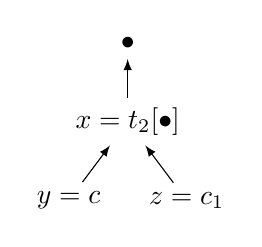
\begin{tikzpicture}[ 
  edge from parent path={(\tikzchildnode\tikzchildanchor) edge [-latex] (\tikzparentnode\tikzparentanchor)},
  level distance=1cm
]
\node (d) {$\bullet$} child{node (a) {$x=t_2[\bullet]$} child{node (b) {$y=c$}} child{node (c)
{$z=c_1$}}};

\end{tikzpicture}
\end{center}
Now each of the environments is represented by a linked list, with the binding
of $x$ shared between them. This is an example of a \emph{shared} environment
~\cite{appel1988optimizing}. This shared, linked structure dates back to the 
first machine for evaluating expressions, Landin's SECD
machine~\cite{landin1964mechanical}.

The drawbacks and advantages of each approach are well known. With a flat
environment, variable lookup can be performed with a simple offset
~\cite{jonesstg,appel1992compiling}. On the other hand, significant
duplication can occur, as we will discuss in Section~\ref{sec:exist}.
With a shared environment, that duplication is removed, but at the cost of
possible link traversal upon dereference. 

As with most topics in compilers and abstract machines, the design space is
actually more complex. For example, Appel and Jim show a wide range of hybrids
~\cite{appel1988optimizing} between the two, and Appel and Shao
~\cite{shao1994space} show an optimized hybrid that aims to achieve the benefits
of both approaches. And as shown in the next section, choice of evaluation
strategy further complicates the picture.

\subsection{Existing Call-by-Need Environments} \label{sec:exist}

Existing call by need machines use flat environments with a heap of
closures~\cite{jonesstg,TIM,johnsson1984efficient,boquist1997grin}. These
environments may contain some combination of primitive values and pointers into the
heap ($p$ below). The pointers and heap implement the memoization of results
required for call by need. Returning to the earlier example, $(\lambda
x.(\lambda y.t) (\lambda z.t_1)) t_2$, we can view a simplified execution state
for this approach when entering $t$ as follows:

\begin{center}
\textbf{Closure}
\begin{align*}
t[x=p_0, y=p_1] \\
\end{align*}
\textbf{Heap}
\begin{align*}
p_0 &\mapsto t_2[\bullet] \\
p_1 &\mapsto \lambda z.t_1[x=p_0] 
\end{align*}
\end{center}

Consider $t_2[\bullet]$, the closure at $p_0$. If it is not in WHNF (this sort
of unevaluated closure is called a
\emph{thunk}~\cite{ingerman1961way,peyton1992implementing}), then if it is
entered in either the evaluation of $t$ or $t_1$, the resulting value will
overwrite the closure at $p_0$. The result of the computation is then shared
with all other instances of $x$ in $t$ and $t_1$. In the case that terms have a
large number of shared variables, environment duplication can be expensive.
Compile-time transformation ~\cite{peyton1992implementing} (tupling arguments)
helps, but we show that the machine can avoid duplication completely.

Depending on $t$, either or both of the closures created for its free variables
may not be evaluated. Therefore, it is possible that the work of creating the
environment for that thunk will be wasted. This waste is well known, and
existing approaches address it by avoiding thunks as much as possible
~\cite{jonesstg,johnsson1984efficient}. Unfortunately, in cases like the above
example, thunks are necessary. We aim to minimize the cost of creating such
thunks.

Thunks are special in another way.  Recall that one advantage of flat
environments is quick variable lookups. In a lazy language, this advantage is
reduced because \emph{a thunk can only be entered once}. After it is entered, it
is overwritten with a value, so the next time that heap location is entered it
is entered with a value and a different environment. Thus, the work to ensure
that the variable lookup is fast is used only once. This is in contrast to
a call by value language, in which every closure is constructed for a value,
and can be entered an arbitrary number of times. 

A more subtle drawback of the flat environment representation is that
environments can vary in size, and thus a value in WHNF can be too large to fit
in the space allocated for the thunk it is replacing. This problem is discussed
in~\cite{jonesstg}, where the proposed solution is to put the value closure in
a fresh location in the heap where there is sufficient room. The original
thunk location is then replaced with an indirection to the value at the freshly
allocated location. These indirections are removed during garbage collection,
but do impose some cost, both in runtime efficiency and implementation
complexity~\cite{jonesstg}.

We have thus far ignored a number of details with regard to current
implementations. For example, the STG machine can split the flat environment, so
that part is allocated on the stack and part on the heap.  The TIM allocates its
flat environments separately from its closures so that each closure is a code
pointer, environment pointer pair~\cite{TIM} while the STG machine keeps
environment and code co-located~\cite{jonesstg}. Still, the basic design
principle holds: a flat environment for each closure allows quick variable
indexing, but with an initial overhead.

To summarize, the flat environment representation in a call by need language is
whenever a term might be needed, the necessary environment is constructed from
the current environment.  This operation can be expensive, and it is wasted if
the variable is never entered. In this work, we aim to minimize this potentially
unnecessary overhead.

Figure~\ref{fig:designspace} depicts the design space relevant to this paper.
There are existing call by value machines with both flat and shared
environments, and call by need machines with flat environments. As far as we are
aware, we are the first to use a shared environment to implement lazy
evaluation. 

It is worth noting that there has been work on lazy machines that effectively use
linked environments, which could potentially be implemented as a shared
environment, e.g., Sestoft's work on Krivine machines~\cite{sestoft}, but none
make the realization that the shared environment can be used to implement
sharing of results, which is the primary contribution of this paper.

\begin{figure}
\begin{tabularx}{\textwidth}{l | X | X}
                & Flat Environment     & Shared Environment \\ \hline
  Call by need  & STG~\cite{jonesstg}, 
                  TIM~\cite{TIM}, 
                  GRIN~\cite{boquist1997grin} 
                & $\mathcal{\mathcal{C} \mskip -4mu \mathcal{E}}$ Machine (this paper) \\
  Call by value & ZAM~\cite{leroy1990zinc}, 
                  SML/NJ~\cite{appel1991standard}
                & ZAM,
                  SECD~\cite{landin1964mechanical}, 
                  SML/NJ \\
\end{tabularx}
\caption{Evaluation strategy and environment structure design space. Each
acronym refers to an existing implementation. Some implementations use multiple
environment representations.}
\label{fig:designspace}
\end{figure}


\section{Cactus Environment Calculus} \label{sec:calc}

This section shows how the shared environment approach can be applied to
call-by-need evaluation. We start with a calculus that abstracts away
environment representation, Curien's calculus of closures, and we show how it
can be modified to force sharing. See Curien's call-by-name calculus of closures
in Figure~\ref{fig:calcclos}. \footnote{Curien calls it a ``lazy'' evaluator, and
there is some ambiguity with the term lazy, but we use the term only to mean
call-by-need. We also remove the condition checking that $i < m$ because we are
only concerned with evaluation of closed terms.}

The LEval rule pushes a closure onto the environment, and the LVar rule indexes
into the environment, entering the corresponding closure. We show in this
section that by removing ambiguity about how the environments are represented,
and forcing them to be represented in a \emph{cactus stack}
~\cite{stenstrom1988vlsi}, we can define our novel call-by-need calculus.

\begin{figure}
\textbf{Syntax}
\begin{align*}
\tag{Term} t &::= i \; | \; \lambda t \; | \; t \; t  \\
\tag{Variable} i &\in \mathbb{N}  \\
\tag{Closure} c &::= t [\rho] \\
\tag{Environment} \rho &::= \bullet \; | \; c \cdot \rho \\
\end{align*}
\textbf{Semantics}
\begin{align*}
\tag{LEval}\inference
{t_1[\rho] {\xrightarrow{* }}_L \lambda t_2[\rho'] }
{t_1 t_3[\rho] \rightarrow_L t_2[t_3[\rho] \cdot \rho'] } 
\end{align*}
\begin{align*}
\tag{LVar} i [c_0 \cdot c_1 \cdot ... c_i \cdot \rho] \rightarrow_L c_i
\end{align*}
\caption{Curien's call-by-name calculus of closures ~\cite{curien1991abstract}}
\label{fig:calcclos}
\end{figure}

To start, consider again the example from Section~\ref{sec:env}, this
time with deBruijn indices: $(\lambda(\lambda t) \; (\lambda t_1)) t_2$.  The
terms $t$ and $t_1$, when evaluated in the closure calculus, would have the
following environments, respectively: 

\begin{center}
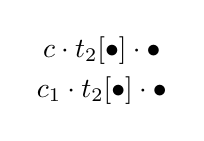
\begin{tikzpicture}
\node {$c \cdot t_2[\bullet] \cdot \bullet$};
\node [yshift=-0.5cm] {$c_1 \cdot t_2[\bullet] \cdot \bullet$};
\end{tikzpicture}
\end{center}

Again, the second closure is identical in each environment.  And again,
we can represent these environments with a shared environment, this time
keeping call-by-need evaluation in mind:
\begin{center}
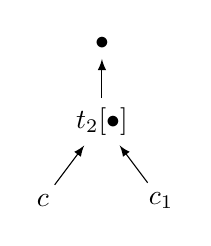
\begin{tikzpicture}[ 
  edge from parent path={(\tikzchildnode\tikzchildanchor) edge [-latex] (\tikzparentnode\tikzparentanchor)},
  level distance=1cm
]
\node (a) {$\bullet$} child{node (d) {$t_2[\bullet]$} child{node (b) {$c$}} child{node (c)
{$c_1$}}};

%\draw let \p1=(a), \p2 =(b), \n1={atan2(\y2-\y1,\x2-\x1)}, \n2={veclen(\y2-\y1,\x2-\x1)}
%  in ($ (a)!0.5!(b) $) ellipse [x radius=\n2/2+10pt, y radius=10pt, rotate=90-\n1];
%\draw let \p1=(a), \p2 =(c), \n1={atan2(\y2-\y1,\x2-\x1)}, \n2={veclen(\y2-\y1,\x2-\x1)}
%  in ($ (a)!0.5!(c) $) ellipse [x radius=\n2/2+10pt, y radius=10pt, rotate=90-\n1];
\end{tikzpicture}
\end{center}
This inverted tree structure seen earlier with the leaves pointing toward the
root is called a \emph{cactus stack} (sometimes called a spaghetti stack or
saguaro stack) \cite{hauck1968burroughs,ichbiah1991rationale}. In this
particular cactus stack, every node defines an environment as the sequence of
closures in the path to the root.  If $t_2[\bullet]$ is a thunk, and is updated
in place with the value after its first reference, then both environments would
contain the resulting value. This is exactly the kind of sharing that is
required by call-by-need, and thus we can use this structure to build a
call-by-need evaluator. This is the essence of the cactus environment calculus
and the cactus environment ($\mathcal{CE}$) machine. 

Curien's calculus of closures does not differentiate between flat and shared
environment representations, and indeed, no calculus that we are aware of has
had the need to. Therefore, we must derive a calculus of closures, forcing the
environment to be shared. Because we can hold the closure directly in the
environment, we choose to replace the standard heap of closures with a
\emph{heap of environments}. To enforce sharing, we extend Curien's
calculus of closures to explicity include the heap of environments, which we
refer to as a \emph{cactus environment}. 

See Figure~\ref{fig:calccact} for the syntax and semantics of the cactus
calculus. Recall that we are only concerned with evaluation of closed terms. The
initial closed term $t$ is placed in a $(t[0],\epsilon[0 \mapsto \bullet])$ tuple, and
evaluation terminates on a value. We use the shorthand $\mu(l,i)=l' \mapsto l''
c \dot e$ to say that looking up the $i$'th element in the linked environment
structure starting at $l$ results in location $l'$, where closure $c$ and
continuing environment $e$ reside. We define two different semantics, one for
call-by-name and one for call-by-need, which makes the connection to
Curien's call-by-name calculus more straightfoward. The rule for application
(MEval and NEval) is identical for both semantics: each evaluates the left hand
side to a function, then binds the variable in the cactus environment, extending
the current environment.

The only difference between this semantics and Curien's is that if we need
to extend an environment multiple times, the semantics \emph{requires}
sharing it among the extensions. This makes no real difference for call-by-name,
but it is needed for the sharing of results in the NVar rule. The explicit
environment sharing ensures that the closure that is overwritten with a value is
shared correctly.

\begin{figure*}
\textbf{Syntax}
\begin{align*}
\tag{Term} t &::= i \; | \; \lambda t \; | \; t \; t  \\
\tag{Variable} i &\in \mathbb{N}  \\
\tag{Closure} c &::= t [l] \\
\tag{Value} v &::= \lambda t [l] \\
\tag{Heap} \mu &::= \epsilon \; | \; \mu [ l \mapsto \rho ] \\
\tag{Environment} \rho &::= \bullet \; | \; c \cdot l \\
\tag{Location} l,f &\in \mathbb{N}  \\
\tag{State} s &::= (c, \mu)
\end{align*}
\textbf{Call-by-Name Semantics}
\begin{align*}
\tag{MEval} \inference
{(t[l], \mu) \xrightarrow{* }_{M} (\lambda t_2[l'], \mu') \quad f \not \in \textnormal{dom}(\mu')}
{(t \; t_3[l], \mu) \rightarrow_{M} (t_2[f], \mu'[f \mapsto t_3[l] \cdot l'])}  
\end{align*}
\begin{align*}
\tag{MVar} \inference 
{\mu(l, i) = l' \mapsto c \cdot l''}
{(i[l],\mu) \rightarrow_M (c,\mu)}
\end{align*}
\textbf{Call-by-Need Semantics}
\begin{align*}
\tag{NEval} \inference
{(t[l], \mu) \xrightarrow{* }_{N} (\lambda t_2[l'], \mu') \quad f \not \in \textnormal{dom}(\mu')}
{(t \; t_3[l], \mu) \rightarrow_{N} (t_2[f], \mu'[f \mapsto t_3[l] \cdot l'])}  
\end{align*}
\begin{align*}
\tag{NVar} \inference
{\mu(l, i) = l' \mapsto c \cdot l'' \quad (c, \mu) \xrightarrow{* }_{N} (v, \mu')}
{(i[l],\mu) \rightarrow_N (v, \mu'[l' \mapsto v \cdot l''])}
\end{align*}
\caption{Cactus calculus syntax and semantics.}
\label{fig:calccact}
\end{figure*}

\subsection{Correctness}

Ariola et al. define the standard call-by-need semantics in
~\cite{ariola1995call}. To show correctness, we show that there is a strong
bisimulation between $\rightarrow_{N}$ and their operational
semantics, $\Downarrow$ (Figure~\ref{fig:cbn}). 

\begin{figure}
\begin{align*}
\tag{Id} \inference
{\langle \Phi \rangle t \Downarrow \langle \Psi \rangle \lambda x.t'}
{\langle \Phi, x \mapsto t, \Upsilon \rangle x \Downarrow \langle \Psi, x
\mapsto \lambda x.t', \Upsilon \rangle \lambda x.t'}
\end{align*}
\begin{align*}
\tag{Abs} \inference 
{}
{\langle \Phi \rangle \lambda x . t \Downarrow \langle \Phi \rangle \lambda x.t}
\end{align*}
\begin{align*}
\tag{App} \inference
{\langle \Phi \rangle t_l \Downarrow \langle \Psi \rangle \lambda 
x.t_n \\ \langle \Psi, x' \mapsto t_m \rangle [x'/x]t_n \Downarrow \langle
\Upsilon \rangle \lambda y.t'}
{\langle \Phi \rangle t_l \; t_m \Downarrow \langle \Upsilon \rangle \lambda y.t'}
\end{align*}
\caption{Ariola et. al's Operational Semantics}
\label{fig:cbn}
\end{figure}

{\theorem \textnormal{(Strong Bisimulation)} $$\xrightarrow{}_{N} \; \sim \;
\Downarrow$$}
We start with a \emph{flattening} relation between a configuration for
$\Downarrow$ and a configuration for $\xrightarrow{}_{N}$. The deBruijn indexed
terms and the standard terms are both converted to terms that use deBruijn
indices for local variables and direct heap locations for free variables. The
flattening relation holds only when both terms are closed under their
corresponding heaps. It holds trivially for the special case of initializing
each configuration with a standard term and its corresponding deBruijn-indexed
term, respectively. The proof is finished by induction on the step relation for
each direction of the bisimulation.

\subsection{Recursion}

Correct sharing for recursive data values, as pointed out in
\cite{ariola1995call}, is not possible without adding explicit recursion. We
return to this issue in Section~\ref{sec:disc}, but note here that adding
explicit recursion to this scheme is left for future work.

\section{$\mathcal{CE}$ Machine} \label{sec:mach}

Using the calculus of cactus environment defined in the previous section, we
derive an abstract machine: the $\mathcal{CE}$ machine\footnote{No relation to
Felleisen and Friedman's CEK machine~\cite{felleisen1986control}}. The syntax
and semantics are defined in Figure~\ref{fig:CEM}. 

\begin{figure*}
\textbf{Syntax}
\begin{align*}
\tag{State} s &::= \langle c, \sigma, \mu, f \rangle \\
\tag{Term} t &::= i \; | \; \lambda t \; | \; t \; t  \\
\tag{Variable} i &\in \mathbb{N}  \\
\tag{Closure} c &::= t [l] \\
\tag{Value} v &::= \lambda t[l] \\
\tag{Heap} \mu &::= \epsilon \; | \; \mu [ l \mapsto \rho ] \\
\tag{Environment} \rho &::= \bullet \; | \; c \cdot l \\
\tag{Context} \sigma &::= \square \; | \; \sigma \; c \;  | \; u:=\sigma \\
\tag{Location} l,u,f &\in \mathbb{N}
\end{align*}
\textbf{Semantics}
\begin{align*}
\tag{Upd}
\langle v, u := \sigma, \mu[u \mapsto c \cdot l], f \rangle 
  &\rightarrow_{\mathcal{CE}}
\langle v, \sigma, \mu[u \mapsto v \cdot l], f \rangle  \\
\tag{Lam}
\langle \lambda t[l], \sigma \; c, \mu, f \rangle 
  &\rightarrow_{\mathcal{CE}}
\langle t[f], \sigma, \mu[f \mapsto c \cdot l], f+1 \rangle  \\
\tag{App}
\langle t \; t'[l], \sigma, \mu, f \rangle
  &\rightarrow_{\mathcal{CE}}
\langle t[l], \sigma \; t'[l], \mu, f \rangle \\
\tag{Var1}
\langle 0[l], \sigma, \mu, f \rangle
  &\rightarrow_{\mathcal{CE}}
\langle c, l := \sigma, \mu, f \rangle 
\; \textnormal{where} \; c \cdot l' = \mu(l)\\
\tag{Var2}
\langle i[l], \sigma, \mu, f \rangle
  &\rightarrow_{\mathcal{CE}}
\langle (i-1)[l'], \sigma, \mu, f \rangle
\; \textnormal{where} \; c \cdot l' = \mu(l)
\end{align*}
\caption{Syntax and semantics of the $\mathcal{CE}$ machine.}
\label{fig:CEM}
\end{figure*}

The machine operates on a similar syntax as the calculus, extended only with a
context to implement the updates from the NVar subderivation ($u:=\sigma$) and
the operands from the NEval subderivation ($\sigma \; c$). We also add $f$
explicitly, which is our fresh heap location. Thus, we now have a 4-tuple, with
initial state $\langle t[0], \square, \epsilon[0=\bullet], 1\rangle$. The four
parts of the tuple are the current closure, the context, the heap, and the fresh
heap location. On the update rule, our current closure is a value, and there is
an update marker as the outermost context. This implies that a variable was
entered, and our current closure represents the corresponding value for that
variable.  Thus, we update the location $u$ that the variable entered, replacing
whatever term was entered with the current closure. The Lam rule takes an
argument off the context and binds it to a variable, allocating a fresh heap
location for the bound variable. This ensures that every instance of the
variable will point to this location, and thus the bound term will only be
evaluated at most once. The App rule simply pushes an argument term in the
current environment. The Var1 rule enters the closure pointed to by the
environment location, while the Var2 rule traverses the cactus environment to
locate the correct closure.  

To get some intuition for the $\mathcal{CE}$ machine and how it works, consider
the depiction in Figure~\ref{fig:state} of its state during evaluation of the
term: $(\lambda a.(\lambda b.b \; a) (\lambda c.c \; a)) ((\lambda i.i) (\lambda
j.j))$. We leave the variable names for readability. For thoroughness, the
occurrences of variable $a$ may be replaced with index $1$, and the rest can be
replaced with index $0$. At this point in the computation, the closure for $a$
is shared, and has been updated with its value. The closure in the context (the
$a$ from the application $c \; a$) now points to the updated value.

\begin{figure}
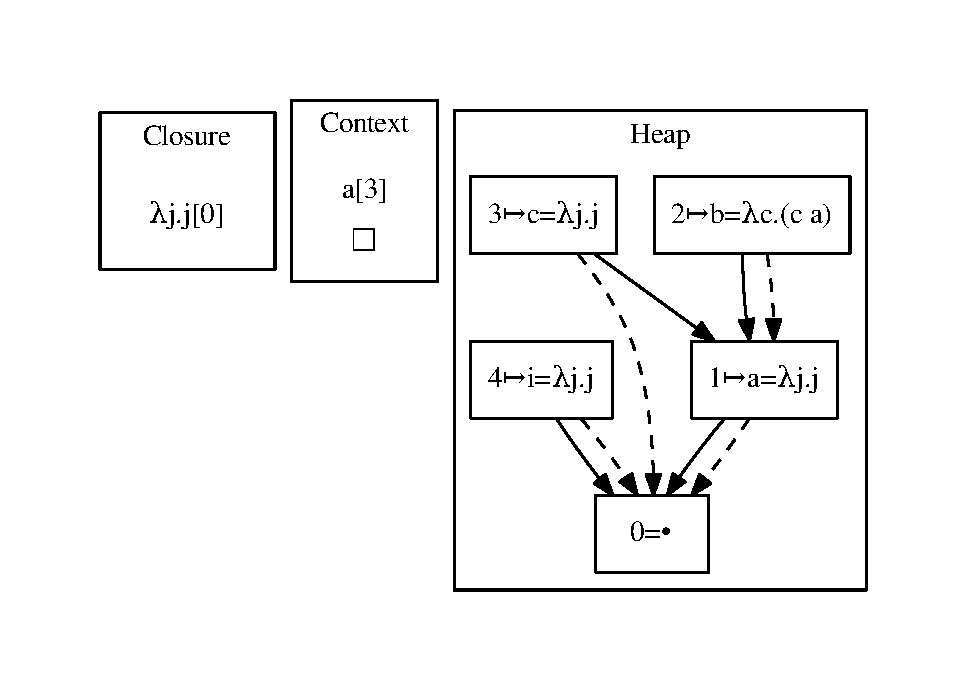
\includegraphics[width=\linewidth]{figures/18.pdf}
The dotted lines represent the environment for the bound closure, and the solid
lines represent the next environment cell:  $t[dotted] \cdot solid$. The
variables are left in for readability, but can be trivially replaced with
deBruijn indices. See Figure~\ref{fig:states} in the Appendix for a
visualization of a number of subsequent machine states. The free Heap location
$f$ is left out to save space.
\caption{$\mathcal{CE}$ machine state example}
\label{fig:state}
\end{figure}

\subsection{Correctness}
We prove that the reflexive transitive closure of the $\mathcal{CE}$ machine
step relation evaluates to a value and heap and empty context iff
$\xrightarrow{}_{M}$ evaluates to the same value and heap.

{\prop \textnormal{(Correctness)} $$(c, \mu) \rightarrow_{M} (v, \mu') \;
\leftrightarrow \; \langle c, \square, \mu \rangle \xrightarrow{*
}_{\mathcal{CE}} \langle v, \square, \mu' \rangle $$} We begin by. 

\section{Implementation} \label{sec:impl}

This section describes how the $\mathcal{CE}$ machine can be mapped directly to
x64 insructions. Specifically, we re-define the three instructions as given by
the TIM~\cite{TIM}: \texttt{TAKE}, \texttt{ENTER}, and \texttt{PUSH}, and
implement them with x64 assembly. We also describe several design decisions, as
well as some optimizations. All implementation and benchmark code is available
at \texttt{http://cs.unm.edu/\textasciitilde stelleg/cem-ifl2015.tar.gz}.

Each closure is represented as a code pointer, environment pointer tuple. The
Context is implemented as a stack, with updates represented as a null pointer,
environment pointer tuple to differentiate them from closure arguments. The
Heap, or cactus environment, is implemented as a heap of environments. 

\subsection{Compilation}
The three instructions are given below, with descriptions of their operational
behaviour. 

\begin{itemize}
\item \texttt{TAKE}: Pops a context item off the stack. If the item is an
update $u:=$, the instruction updates the location $u$ with the current closure.
If it is an argument $c$, the instruction binds the closure $c$ to the fresh
location in the cactus environment.
\item \texttt{ENTER i}: Enters the closure defined by variable index \texttt{i},
the current environment pointer, and the current cactus environment.  \item
\texttt{PUSH m}: Pushes the code location \texttt{m} along with the
current environment pointer. 
\end{itemize}

These operations correspond directly to lambda terms, and to the transition
functions of the $\mathcal{CE}$ machine. The mapping from lambda terms can be
seen in Figure~\ref{fig:cemcompile}, which defines the compiler. Unlike the TIM,
our version of \texttt{TAKE} doesn't have an arity; we compile a sequence of
lambdas as a sequence of \texttt{TAKE} instructions. While we are not aware of a
direct performance comparison between the approaches, we do not see any inherent
reason that a number of inlined \texttt{TAKE} instructions should be slower than
a \texttt{TAKE n} instruction.  Similarly, the \texttt{ENTER i} instruction can
be implemented either as a loop or unrolled, depending on \texttt{i}, and more
performance comparisons are needed to determine the trade off between code size
and speed.

\begin{figure}
\begin{align*} C[t \; t'] &= \texttt{PUSH}\;label_{C[t']}:C[t] \concat C[t'] \\
C[\lambda.t] &= \texttt{TAKE}:C[t] \\
C[i] &= \texttt{ENTER} \; i
\end{align*}
\caption{$\mathcal{CE}$ machine compilation scheme. $C$ compiles a sequence of
instructions from a term. The $label$ represents a code label: each instruction
is given a unique label. The $:$ operator denotes prepending an item to a
sequence and $\concat$ denotes concatenating two sequences.}
\label{fig:cemcompile}
\end{figure}

We compile to x64 assembly. Each of the three instructions is mapped onto
x64 instructions with a macro. The \texttt{PUSH} instruction is particularly
simple, consisting of only two x64 instructions (two \texttt{push}es, one for
the code pointer and one for the environment pointer). This is actually an
important point: \emph{thunk creation is only two hardware instructions,
regardless of environment size}.  

\subsection{Machine Literals and Primitive Operations}

Following Sestoft ~\cite{sestoft} we extend the $\mathcal{CE}$ machine to
include machine literals and primitive operations. Figure~\ref{fig:extsyntax}
shows the parts of syntax and semantics that are new or modified. 

\begin{figure}
\textbf{Syntax}
\begin{align*}
\tag{Term}    t &::= i \; | \; \lambda t \; | \; t \; t | \; m \\
\tag{Machine} m &::= n \; | \; op \\
\tag{Integer} n &\in \mathbb{I} \\
\tag{PrimOp} op &::= + \; | \; - \; | \; * \; | \; \; / \;\; | \; = \; | \; > \; | \; < \\
\tag{Value} v &::= \lambda t[l] \; | \; m[l] \\
\end{align*}
\textbf{Integer and Primop Semantics}
\begin{align*}
\tag{Int}
\langle n[l], \sigma \; c, \mu, k \rangle
  &\rightarrow_{\mathcal{CE}}
\langle c, \sigma \; n[l], \mu, k \rangle \\
\tag{Op} 
\langle op[l], \sigma \; n' \; n, \mu, k \rangle
  &\rightarrow_{\mathcal{CE}}
\langle op(n',n)[l], \sigma, \mu, k \rangle
\end{align*}
\caption{Extensions to the syntax and semantics of the $\mathcal{CE}$ machine.}
\label{fig:extsyntax}
\end{figure}

\subsection{Omitted Extensions}

Our implementation omits a few other standard extensions. Here we address some
of these omissions.

Data types are a common extension that we omit ~\cite{jonesstg,boquist1997grin}.
We take the approach of Sestoft ~\cite{sestoft} that these can be efficiently
implemented with pure lambda terms. Consider a list data type (in Haskell
syntax): \texttt{data List a = Cons a (List a) | Nil}. This can be represented
in pure lambda terms with $Cons = \lambda h.\lambda t.\lambda c.\lambda n.c \; h
\; t$ and $Nil = \lambda c.\lambda n.n$. 

Let bindings are another term commonly included in most functional language
compilers, even in the internal representation ~\cite{boquist1997grin,jonesstg}.
Non-recursive let is syntactic sugar for a lambda binding and application, and
thus we treat it as such. This approach helps to ensure that we are capable of
compiling arbitrary lambda terms, while some approaches require pre-processing
~\cite{sestoft,TIM}.

Recursive let bindings are another omission. Here we follow Rozas
~\cite{rozas1992taming}: if it can be represented in pure lambda terms, it should
be. Thus, we implement recursion using the standard Y combinator. In the case of
mutual recursion, we use the Y combinator in conjunction with a tuple of the
mutually recursive functions. Without the appropriate
optimizations ~\cite{rozas1992taming}, this approach has a large overhead, as we
discuss in Section~\ref{sec:res}.

There is a common pattern in these omissions: if recursion, let bindings, data
types, etc., can be represented with pure lambda calculus, then optimized to
achieve equal performance to those that represent them explicitly, then do so.
This allows opportunity for application of general purpose optimizations that
may optimize data types, but also will optimize normal function applications
that share some properties with data types.

\subsection{Optimizations}

The $\mathcal{CE}$ implementation described in the previous section is a
completely unoptimized implementation. For example, there is no effort to
discover global functions to avoid costly jumps to pointers in the heap
~\cite{jonesstg}. Indeed, every variable reference will look up the code pointer
in the shared environment and jump to it. There is also no implementation of 
control flow analysis as used by Rozas to optimize away the Y combinator.  Thus,
every recursive call exhibits the large overhead involved in re-calculating the
fixed point of the function.  

We do, however, implement a couple of basic optimizations, primarily to reduce
the load on the heap:

\begin{itemize}
\item \texttt{POP}: A \texttt{TAKE} instruction can be converted to a \texttt{POP}
instruction that throws away the operand on the top of the stack if there are no
variables bound to the $\lambda$ term in question. For example, the function
$\lambda x.\lambda y.x$ can be implemented with \texttt{TAKE}, \texttt{POP},
\texttt{ENTER 0}.  
\item \texttt{ENTERVAL}: An \texttt{ENTER} instruction, when entering a
closure that is already a value, should not push an update marker onto the
stack. This shortcut prevents unnecessary writes to the stack and heap
~\cite{jonesstg,lkm,sestoft}.  
\end{itemize}

\subsection{Garbage Collection}

We implement a simple mark and sweep garbage collector with the property
that it does not require two spaces, due to the constant sized closures in the
heap, allowing a linked list representation for the free cells.  Indeed,
while the abstract machine from Section~\ref{sec:mach} increments a free heap
counter, the actual implementation uses the next free cell in the linked list.

Because the focus of this paper is not on the performance of garbage collection,
we ensure the benchmarks in Section~\ref{sec:eval} are not dominated by GC time.
Still, there is a significant connection between closure representation and
garbage collection ~\cite{appel1988optimizing}, and we discuss this further in
Section~\ref{sec:disc}. 


\section{Performance Evaluation} \label{sec:eval}

This section describes experiments that asses the strengths and weaknesses of
the $\mathcal{CE}$ machine. We evaluate using benchmarks from the \texttt{nofib}
benchmark suite. Because we have implemented only machine integers, and must
translate the examples by hand, we use a subset of the \texttt{nofib} suite that
does not use floating point values or arrays. Ideally, we would have a compiler
from Haskell to our intermediate representation. We discuss the possibility of a
Haskell compiler using our implementation as a backend in
Section~\ref{sec:disc}. A list of the benchmarks used and a brief description is
given in Figure~\ref{fig:bench}.

\begin{figure}
\begin{itemize}
\item \textbf{exp3:} A peano arithmetic benchmark. It computes $3^8$ in
peano arithmetic, and prints the result. 
\item \textbf{queens:} Computes the number of solutions to the nqueens problem
for an n by n board.
\item \textbf{primes:} A simple primes sieve that computes the nth prime.
\item \textbf{digits-of-e1:} A calculation of the digits of $e$ using continued
fractions. Computes the first n digits of $e$.
\item \textbf{digits-of-e2:} Another calculation of the digits of $e$ using an
infinite series. Computes the first n digits of $e$. 
\item \textbf{fib:} Naively computes the n'th Fibonacci number.
\item \textbf{fannkuch:} A counting benchmark counting the number of reverses of
a subset of a list.
\item \textbf{tak:} A synthetic benchmark involving basic recursion.
\item \textbf{expexp:} Our own synthetic benchmark, using church numerals to
calculate $3^8-3^8$. We add this example to compare implementations on
equivalent pure lambda terms.
\end{itemize}
\caption{Description of Benchmarks}
\label{fig:bench}
\end{figure}

We compare the $\mathcal{CE}$ machine to two existing implementations:

\begin{itemize}
\item GHC: The Glasgow Haskell compiler. A high performance, optimizing compiler
based on the STG machine \cite{jonesstg}.
\item UHC: The Utrecht Haskell compiler. An optimizing compiler based on the
GRIN machine \cite{boquist1997grin, dijkstra2009architecture}.
\end{itemize}

We use GHC version 7.8.3 and UHC version 1.1.5. We compile with both -O0 and
-O3, and show the results for both. For GHC, we use the -H flag from the runtime
system options to set the default heap size to the same value as the
$\mathcal{CE}$ machine (1G) to avoid the measuring the performance of GC
implementations. The tests were run on an Intel(R) Xeon(R) CPU E5-4650L @
2.60GHz, running Linux version 3.16. 

\subsection{Results} \label{sec:res}

Figure~\ref{fig:res} gives the benchmark results.  In general, we are
outperformed by GHC, sometimes significantly, and we outperform UHC. We
spend the remainder of the section analyzing these performance differences.

\begin{figure*}
\centering
\begin{tabularx}{\textwidth}{l | X | X | X | X | X}
& $\mathcal{\mathcal{C} \mskip -4mu \mathcal{E}}$ & GHC -O0 & UHC -O0 & GHC -O3 & UHC -O3 \\
\hline
\texttt{exp3 8} & 1.530 & 1.176 & 3.318 & 1.038 & 2.286 \\
\texttt{tak 16 8 0} & 0.366 & 0.146 & 1.510 & 0.006 & 1.416 \\
\texttt{primes 1500} & 0.256 & 0.272 & 1.518 & 0.230 & 1.532 \\
\texttt{queens 9} & 0.206 & 0.050 & 0.600 & 0.012 & 0.598 \\
\texttt{fib 35} & 2.234 & 0.872 & 10.000 & 0.110 & 8.342 \\
\texttt{digits-of-e1 1000} & 3.576 & 1.274 & 21.938 & 0.118 & 22.010 \\
\texttt{digits-of-e2 1000} & 0.404 & 0.792 & 3.430 & 0.372 & 3.278 \\
\texttt{fannkuch 8} & 0.560 & 0.084 & 2.184 & 0.048 & 2.196 \\
\end{tabularx}
\caption{Machine Literals Benchmark Results. Measurement is wall clock time,
units are seconds. Times averaged over 5 runs.}
\label{fig:res}
\end{figure*}

There are many optimizations built into the abstract machine underlying GHC,
but profiling indicates that three in particular lead to much of the performance
disparity: 

\begin{itemize}
\item \textbf{Register allocation:} The $\mathcal{\mathcal{C} \mskip -4mu \mathcal{E}}$ machine has no register
allocator. In contrast, by passing arguments to functions in registers, GHC
avoids much heap thrashing.
\item \textbf{Unpacked literals:} This allows GHC to keep machine literals
without tags in registers for tight loops. In contrast, the $\mathcal{\mathcal{C} \mskip -4mu \mathcal{E}}$
machine operates entirely on the stack, and has a code pointer associated with
every machine literal. 
\item \textbf{Y combinator:} Because recursion in the $\mathcal{\mathcal{C} \mskip -4mu \mathcal{E}}$ machine is
implemented with a Y combinator, it performs poorly. This could be alleviated
with CFA-based techniques, similar to those used in ~\cite{rozas1992taming}. 
\end{itemize}

Lack of register allocation is the primary current limitation of the $\mathcal{\mathcal{C} \mskip -4mu \mathcal{E}}$
machine. The STG machine pulls the free variables into registers, allowing tight
loops with everything kept in registers. However, it is less clear how to
effectively allocate registers in a fully shared environment setting.
That said, we believe being lazier about register allocation, e.g., not loading
values into registers that may not be used, could have some performance benefits.

To isolate the effect of register allocation and unpacked machine
literals, we replace machine integers with Church numerals in a compatible
subset of the evaluation programs. Figure~\ref{fig:res-church}
shows the performance results with this modification, which are much improved,
with the $\mathcal{\mathcal{C} \mskip -4mu \mathcal{E}}$ machine occasionally even outperforming optimized GHC.

\begin{figure*}
\centering
\begin{tabularx}{\textwidth}{l | X | X | X | X | X}
& $\mathcal{\mathcal{C} \mskip -4mu \mathcal{E}}$ & GHC -O0 & UHC -O0 & GHC -O3 & UHC -O3 \\
\hline
\texttt{tak 14 7 0} & 1.610 & 2.428 & 7.936 & 1.016 & 7.782 \\
\texttt{primes 32} & 0.846 & 1.494 & 4.778 & 0.666 & 5.290 \\
\texttt{queens 8} & 0.242 & 0.374 & 1.510 & 0.154 & 1.508 \\
\texttt{fib 23} & 0.626 & 0.940 & 5.026 & 0.468 & 5.336 \\
\texttt{digits-of-e2 6} & 0.138 & 1.478 & 5.056 & 0.670 & 5.534 \\
\texttt{fannkuch 7} & 0.142 & 0.124 & 0.796 & 0.040 & 0.808 \\
\end{tabularx}
\caption{Church Numeral Benchmark Results. Measurement is wall clock time, 
units are seconds. Times averaged over 5 runs.}
\label{fig:res-church}
\end{figure*}

Next, we consider the disparity due to the Y-combinator, by running a simple
exponentiation example with Church numerals, calculating $3^8 - 3^8 = 0$. In
this case, the $\mathcal{\mathcal{C} \mskip -4mu \mathcal{E}}$ machine significantly outperform both GHC and UHC,
as seen in Figure~\ref{fig:res-church-exp} .

\begin{figure*}
\begin{tabularx}{\textwidth}{l | X | X | X | X | X}
& $\mathcal{\mathcal{C} \mskip -4mu \mathcal{E}}$ & GHC -O0 & UHC -O0 & GHC -O3 & UHC -O3 \\
\hline
\texttt{pow 3 8} & 0.564 & 1.994 & 4.912 & 0.906 & 4.932 \\
\end{tabularx}
\caption{Church Numeral Exponentiation Benchmark Results. Measurement is wall clock time, 
units are seconds. Times averaged over 5 runs.}
\label{fig:res-church-exp}
\end{figure*}

These results give us confidence that by adding the optimizations mentioned
above, among others, the $\mathcal{\mathcal{C} \mskip -4mu \mathcal{E}}$ machine has the potential to be the
basis of a real-world compiler. We discuss how some of these optimizations can
be applied to the $\mathcal{\mathcal{C} \mskip -4mu \mathcal{E}}$ machine in Section~\ref{sec:disc}.

\subsection{The Cost of the Cactus}

Recall that variable lookup is linear in the index of the variable, following
pointers until the index is zero. As one might guess, the lookup cost is high.
For example, for the queens benchmark without any optimizations, variable lookup
took roughly $80-90\%$ of the $\mathcal{\mathcal{C} \mskip -4mu \mathcal{E}}$ machine runtime, as measured
by profiling. Much of that cost was for lookups of known combinators, however,
so for the benchmarks above we added the inlining mentioned in the previous
section. Still, even with this simple optimization, variable lookup takes
roughly $50\%$ of execution time. There is some variation across benchmarks, but
this is a rough approximation for the average cost. We discuss how this cost
could be addressed in future work in Section~\ref{sec:disc}.



\section{Discussion} \label{sec:disc}

While we have presented some of the related work throughout the paper, we use
this section to further address related work. We also discuss a number of
possibilities for future work, motivated by current drawbacks and inspired by
related work. 

\subsection{Closure Representation}

Appel and Shao \cite{shao1994space} and Appel and Jim \cite{appel1988optimizing}
both cover the design space for closure representation, and develop a particular
approach, called \emph{safely linked closures}. Their approach uses flat
closures when there is no duplication, and link in a way that preserves
liveness, to prevent violation of the \emph{safe for space complexity} (SSC)
rule \cite{appel2006compiling}.

Unfortunately, the technique from Appel and Shao is not directly applicable to
call by need languages, like those used in this paper. To see why, consider the
following example taken from Section 2 of their paper
\cite{appel1988optimizing}:
\begin{verbatim}
fun f(h, u, v, w) = 
  let fun g() = 
    let x = h(u ,v)
        y = h(x, v)
        z = h(y, w)
     in z
    end
   in g
  end
\end{verbatim}
The point made by the authors is that for a call by value language, the compiler
can and should free the variable \texttt{u} after the first call to \texttt{h};
it is no longer live. In a call by need variant of this program, however, we
cannot know if \texttt{u} will be needed until either it is forced after
\texttt{x,y} and \texttt{z} are all forced, or it becomes unreachable. In other
words, we cannot say in general when \texttt{u} will be unreachable, and so we
cannot apply the technique as described in the paper.

In the future we should be able to apply some of the basic ideas as described in
Appel and Jim \cite{appel1988optimizing}. In particular, we aim to flatten the
cactus structure when possible. If we can either prove that a particular segment
of the cactus structure will not branch, or provide a transformation to
encourage such environments, then we can flatten certain parts of the cactus
environment, reducing space usage and variable lookup time. Many of the
underlying ideas of the \emph{safely linked closures} \cite{shao1994space}
should be applicable here. We propose such investigation for future work.

Another point is space safety for the current machine. As pointed out by Appel
and Shao, the naive linked representation is not really safe for space at all;
many variables that should be freed are kept live because they reside in the linked
environment of a particular closure, despite not being free variables of said
closure. As a simple partial fix, we use the standard procedure of compiling an
info table for each closure code pointer, allowing the garbage collector to mark
each closure in the cactus environment as live or not live according to the free
variables of closures, not just reachability on the cactus stack. Then, while
the environment cell itself cannot be freed, the closure in the cell can,
preventing a real space leak and incurring only a small constant space cost.

Consider also the application of Appel et al.'s ideas regarding hybrid
flat-shared environments. While the cactus stack structure is at least partially
linked, there \emph{can} be flat sections. We would need to ensure that flat
sections (e.g.\ functions with arity $> 1$) were detected correctly, and the
ENTER rule was extended to handle it correctly, but it should be possible. The
hybrid approach would allow proper sharing with simple offsets when possible,
improving performance for variable lookup. We consider this a promising area for
future work.

\subsection{Eval/Apply vs. Push/Enter}

Marlow and Peyton Jones' paper describes two approaches to the implementation of
function application: eval/apply, where the function is evaluated and then
passed the necessary arguments, and push/enter, where the arguments are pushed
onto the stack and the function code is entered \cite{marlow2004making}.

They conclude that despite push/enter being a standard approach to lazy
machines, eval/apply performs better. Therefore, our choice of a push/enter
model requires some justification.  As a first point, the current implementation
has no fixed arity functions: each function is of arity one; functions with
multiple arguments are represented as curried functions of one argument.  This
property makes some of the arguments made by Marlow and Peyton Jones not apply
to our machine. We address a few remaining points from their ``advantages of
eval/apply'' list ~\cite{marlow2004making}:

\begin{itemize}
\item \emph{Eval/apply easier to map to a portable assembly language, such as C or
C{-}-.} We concede this is likely the case for existing portable assembly
languages, but note that our implementation is straightforward, with apply
consisting of only two assembly instructions.
\item \emph{No need to distinguish return addresses from heap pointers.} Because
of our standard sized closures, our implementation of push/enter does not suffer
this issue.
\item \emph{No tagging for non-pointers.} We do not use tagging, and so are not
affected by this arguments.
\item \emph{No need for the \texttt{Su} pointer}. This is a fundamental
difference in approach; our implementation \emph{only} needs the \texttt{Su}
pointer (the pointer into the cactus stack). 
\item \emph{Arity matching burden on caller makes \texttt{foreign} calls more
straight forward.} The wrapper required for foreign calls in our push/enter
approach is trivial.
\item \emph{Unknown functions called with number of arguments matching arity can
have arguments passed in registers.} We discuss this issue in
Section~\ref{sec:alloc}.  
\end{itemize}

\subsection{Collapsed Markers}
Friedman et al.\ show how a machine can be designed to prevent multiple adjacent
update markers being pushed onto the stack \cite{lkm}.  This property is
desirable because multiple adjacent update markers will all be updated with the
same value. Furthermore, they give examples showing that in some cases, these
redundant update markers can cause an otherwise constant-spaced stack to grow
unbounded. To achieve what they call collapsed markers, they add a layer
of indirection between heap locations and closures. We propose a similar
approach, but without the performance hit induced by an extra layer of
indirection: upon a variable dereference, check if the top of the stack is an
update. If it is, instead of pushing a redundant update marker onto the stack,
replace the closure in the heap at the desired location with an update marker.
Then, the variable dereference rule must have a check for an update marker upon
dereference, and will update accordingly. We have begun to implement this
optimization, but leave the full implementation and description for future work.

\subsection{Register Allocation} \label{sec:alloc}
One advantage of flat environments is that register allocation is
straightforward \cite{appel2006compiling, jonesstg, terei2010llvm}. It is less
obvious on how to approach register allocation with the $\mathcal{CE}$ machine.
This remains an area for future work. However, we argue that \emph{only strict
free variables should be loaded into registers}. That is to say, the environment
variables may not be used, and only the ones we are sure will be used should be
loaded into registers. The rest should be loaded on demand. Whether or not this
is the case should make for interesting future work.

\subsection{Historical Note}
Given that lazy evaluation is three or four decades old, and shared environments
about five, it might seem surprising that the connection between the two made in
this paper was not discovered earlier. We speculate that lazy evaluation via
graph reduction of supercombinators was so successful that the field firmly
committed to that approach. For good reason, too: GHC is a very high
performance compiler, sometimes achieving higher performance than
implementations in lower level languages, such as C \cite{mainland2013exploiting}. 



\section{Conclusion} \label{sec:conc}

We would like the reader to take a few key points from this paper. First, a
shared environment, explicitly represented as a cactus stack, is a natural
way to share the results of computation as required by lazy evaluation. Second,
this approach can be formalized in both big-step and small-step semantics.
Third, the abstract machine can be implemented as a compiler in a
straightforward way, yielding performance comparable to existing
implementations. 


\section{Acknowledgments}
Sandia is a multiprogram laboratory operated by Sandia Corporation, a Lockheed Martin Company, for the United States Department of Energy’s National Nuclear Security Administration under contract DE-AC04-94AL85000.

% We recommend abbrvnat bibliography style.
\bibliographystyle{abbrvnat}
\bibliography{annotated}

\section{Appendix}
\begin{figure*}
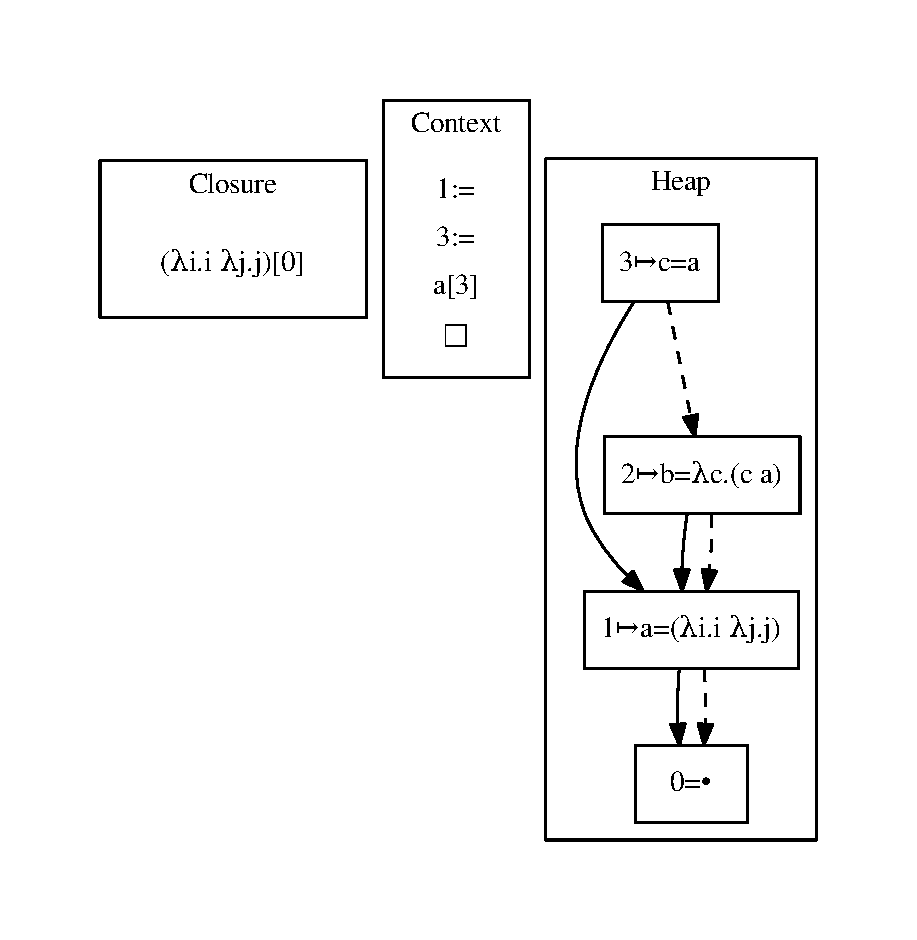
\includegraphics[width=\linewidth/3]{figures/12.pdf}
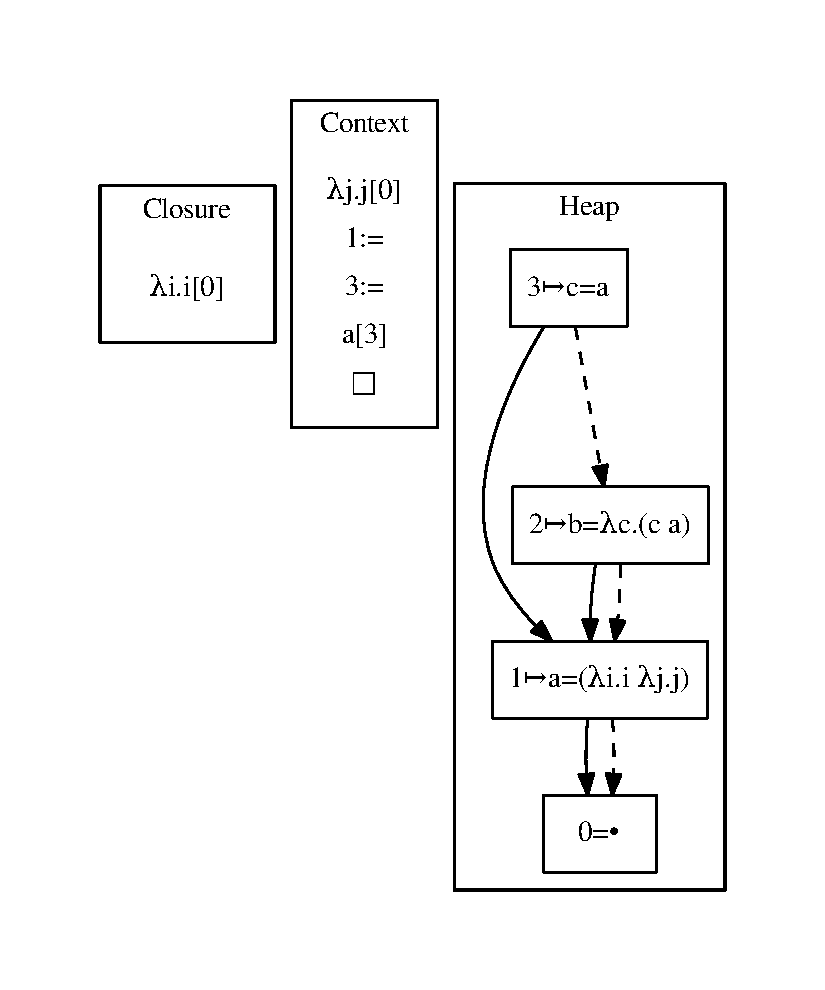
\includegraphics[width=\linewidth/3]{figures/13.pdf}
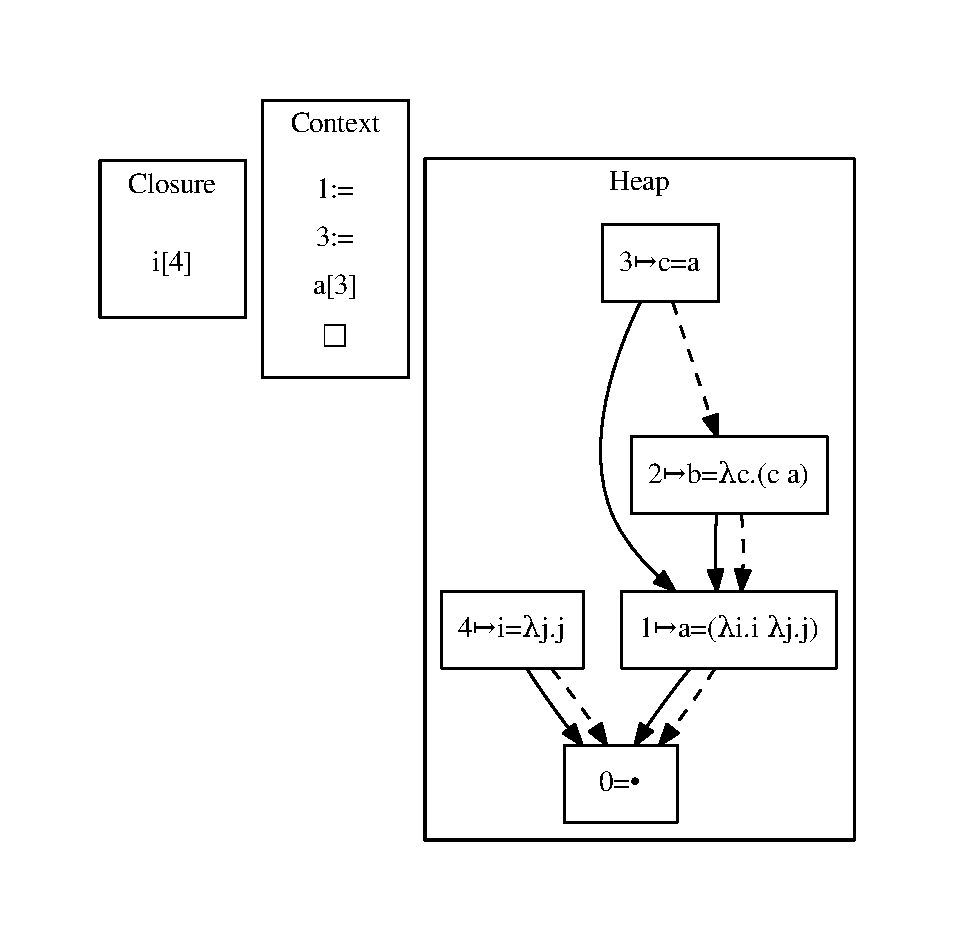
\includegraphics[width=\linewidth/3]{figures/14.pdf}
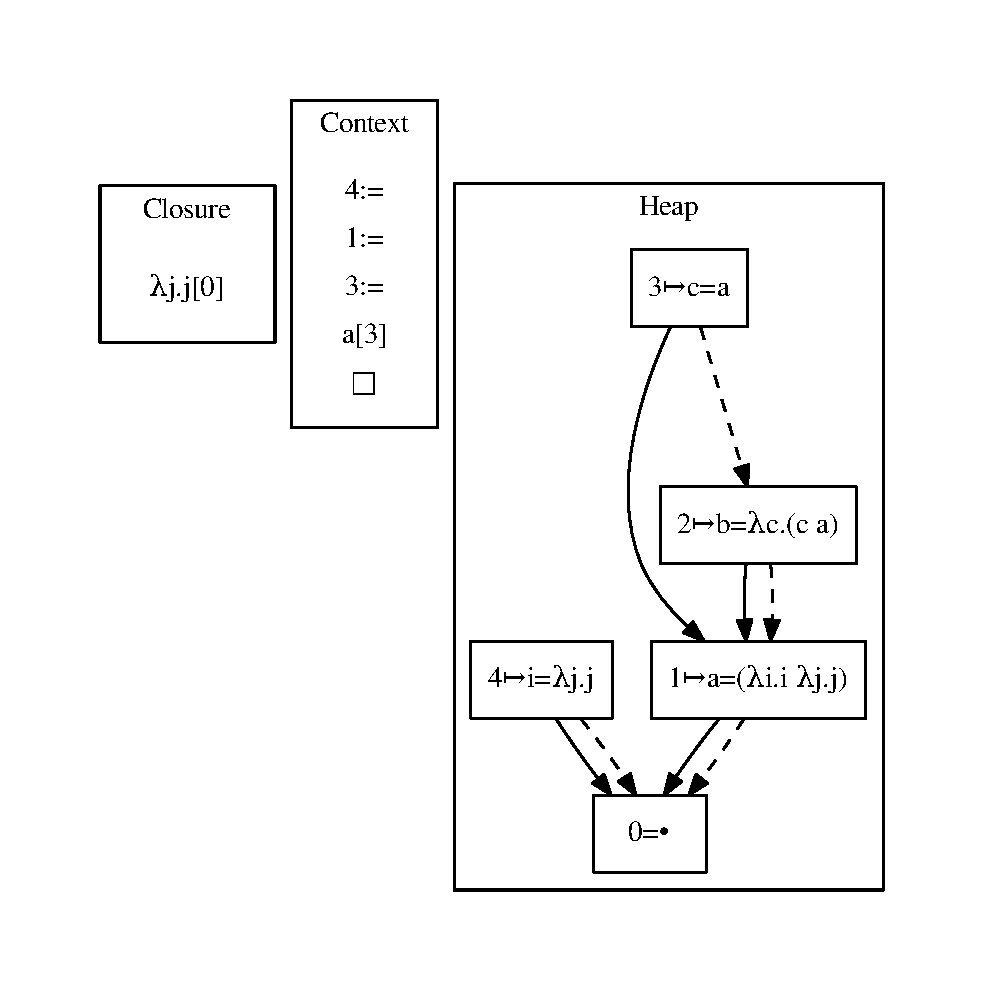
\includegraphics[width=\linewidth/3]{figures/15.pdf}
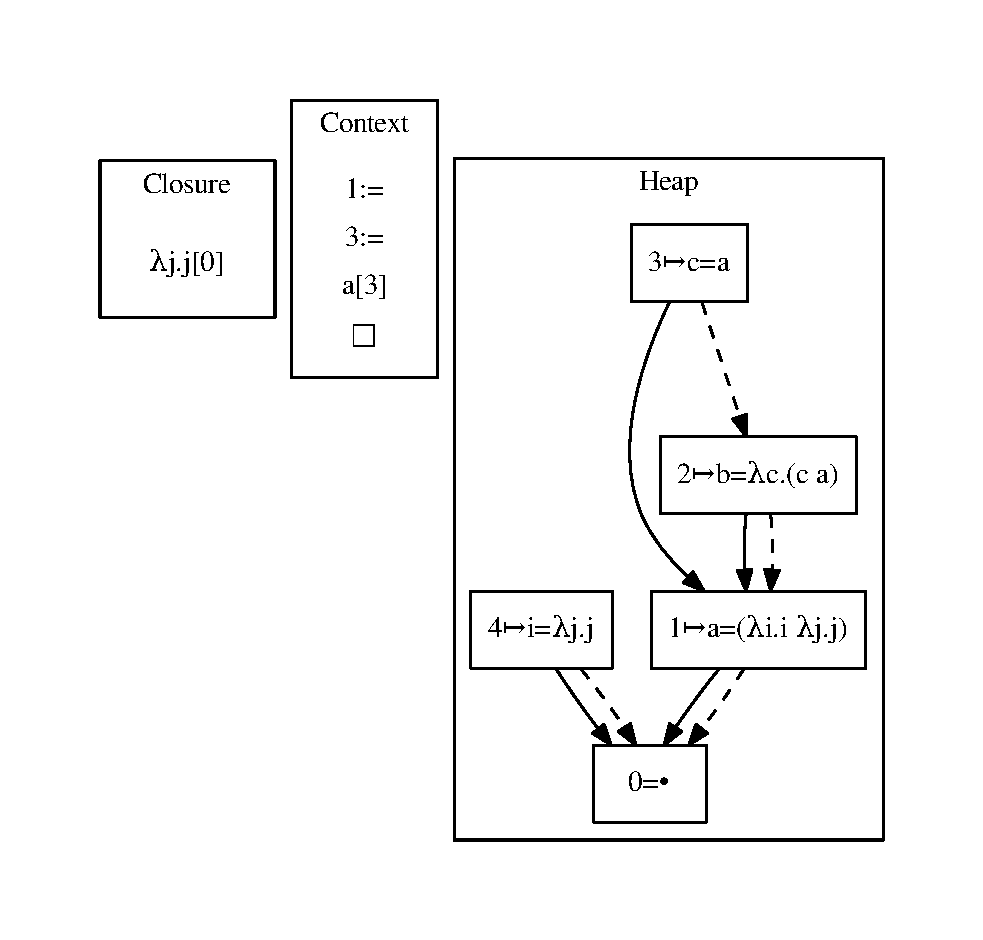
\includegraphics[width=\linewidth/3]{figures/16.pdf}
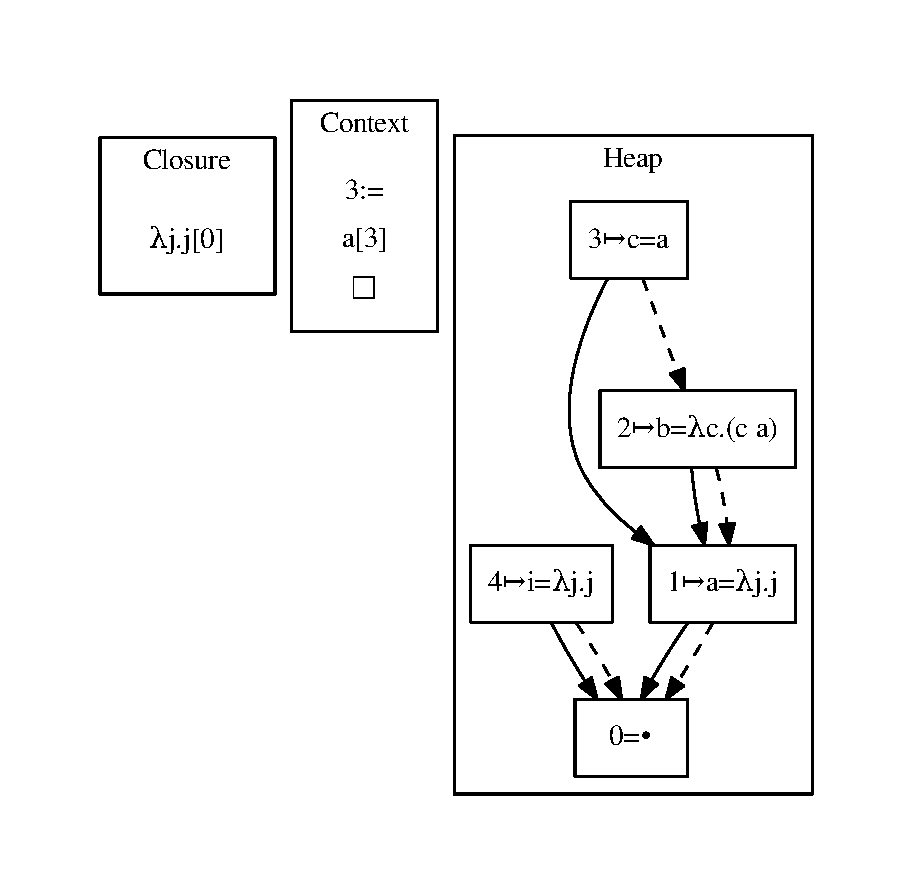
\includegraphics[width=\linewidth/3]{figures/17.pdf}
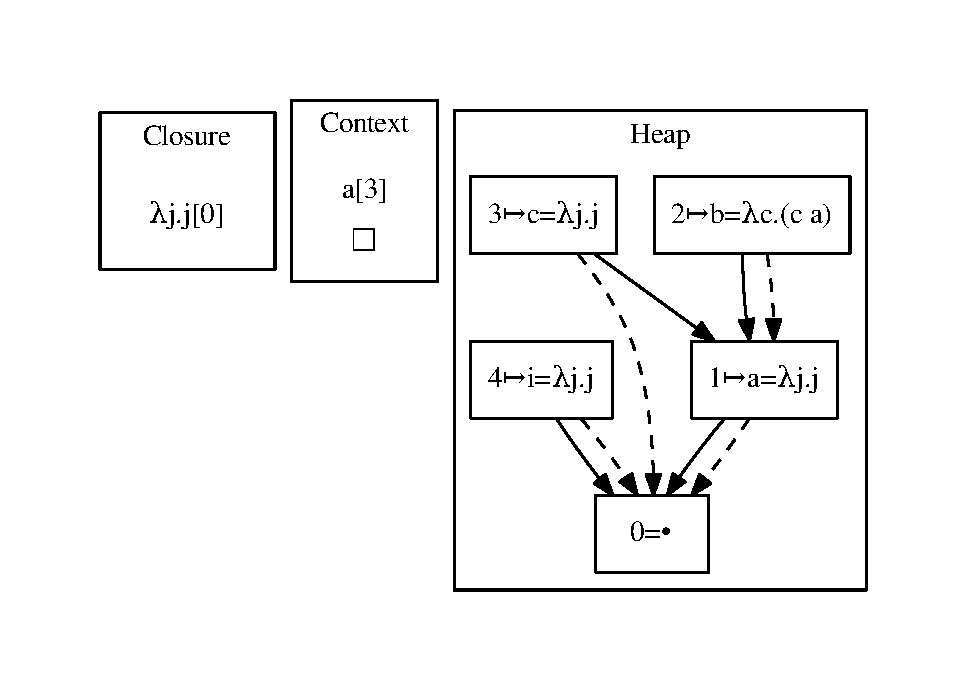
\includegraphics[width=\linewidth/3]{figures/18.pdf}
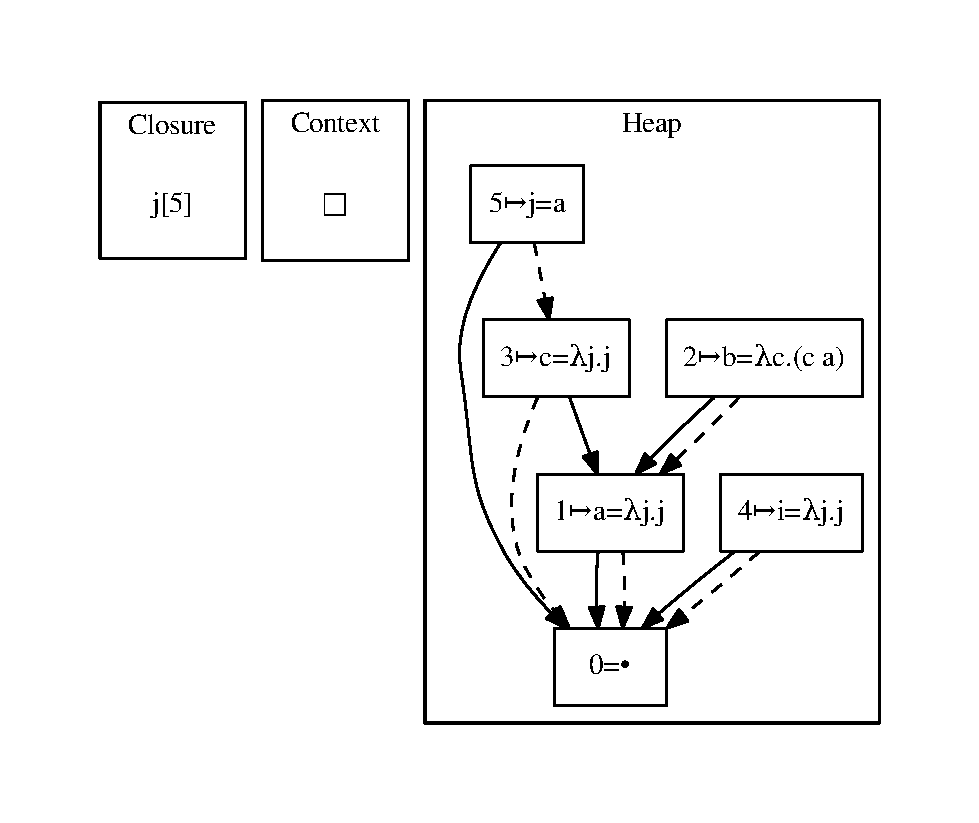
\includegraphics[width=\linewidth/3]{figures/19.pdf}
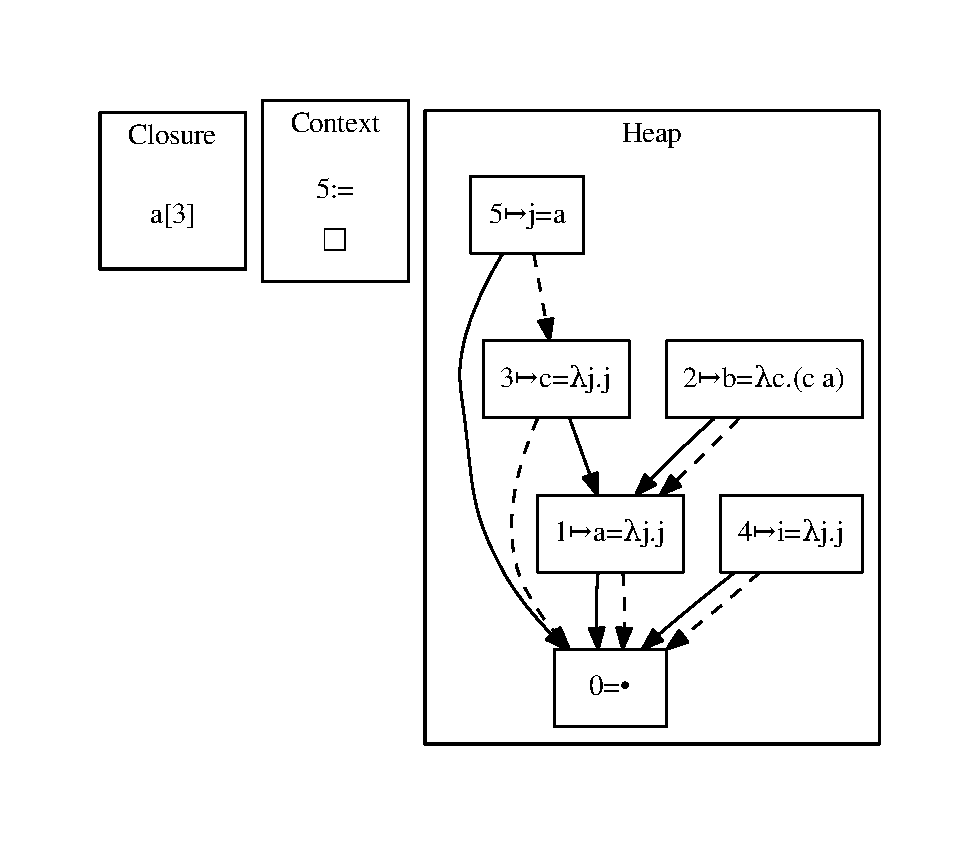
\includegraphics[width=\linewidth/3]{figures/20.pdf}
\caption{An example sequence of machine states during the evaluation of the term
$(\lambda a.(\lambda b.b \; a) (\lambda c.c
\; a)) ((\lambda i.i) (\lambda j.j))$. Order is left to right, top to bottom.
The free heap location $f$ is left out to save space.}
\label{fig:states}
\end{figure*}

\end{document}
